\documentclass{beamer}

\usepackage[T1]{fontenc}
\usepackage{inputenc}

\usepackage{amsmath}
\usepackage{listings}
\lstset{
  basicstyle=\footnotesize,
  language=Caml,
  showstringspaces=false,
}


\usetheme{Boadilla}
\usecolortheme{dolphin}
\useoutertheme{infolines}


\setbeamertemplate{footline}
{
  \leavevmode%
  \hbox{%
  \begin{beamercolorbox}[wd=.333333\paperwidth,ht=2.25ex,dp=1ex,center]{author in head/foot}%
    \usebeamerfont{author in head/foot}\insertshortauthor%~~\beamer@ifempty{\insertshortinstitute}{}{(\insertshortinstitute)}
  \end{beamercolorbox}%
  \begin{beamercolorbox}[wd=.333333\paperwidth,ht=2.25ex,dp=1ex,center]{title in head/foot}%
    \usebeamerfont{title in head/foot}\insertshorttitle
  \end{beamercolorbox}%
  \begin{beamercolorbox}[wd=.333333\paperwidth,ht=2.25ex,dp=1ex,right]{date in head/foot}%
    \usebeamerfont{date in head/foot}\insertshortdate{}\hspace*{2em}
    \insertframenumber{} / \inserttotalframenumber\hspace*{2ex}
  \end{beamercolorbox}}%
  \vskip0pt%
}


\newcommand{\TODO}{{\color{red}\bf [TODO]}}


\title{Trusted Execution Enviroments}
\author{Maxime Puys}
\date{\today}


\begin{document}

\begin{frame}
    \maketitle
\end{frame}

\begin{frame}
    \frametitle{Disambiguation 1/3}

    \begin{block}{TEE}
        {\bf Trusted Execution Environment} -- Secured area in a device where execution is assumed safe (see later).
    \end{block}
    \vfill
    \begin{block}{TCG}
        {\bf Trusted Computing Group} -- Not-for-profit organization formed to develop, define and promote [...] global industry standards, supportive of a hardware-based root of trust, for interoperable trusted computing platforms.
    \end{block}
\end{frame}

\begin{frame}
    \frametitle{Disambiguation 2/3}
    \begin{block}{TPM}
        {\bf Trusted Plateform Module} -- Paradigm proposed by the TCG to obtain a TEE through {\em Static Root of Trust Measurement} (see later).
    \end{block}
    \vfill
    \begin{block}{TCB}
        {\bf Trusted Computing Base} -- Smallest amount of code (and hardware, people, processes, etc.) that you must trust in order to meet your security requirements.
    \end{block}
\end{frame}

\begin{frame}
    \frametitle{Disambiguation 3/3}
    \begin{block}{TCE}
        {\bf Trusted Computing Environment} -- Same as TEE but the name is influenced by TCG.
    \end{block}
    \vfill
    \begin{block}{TE}
        {\bf Trusted Environment} -- TEE for thoose under time pressure.
    \end{block}
\end{frame}

\begin{frame}
    \tableofcontents
\end{frame}

\section{What is a TEE?}

\begin{frame}
    \frametitle{TEE in the secure application ecosystem of today}

    \begin{figure}[htb]
        \centering
        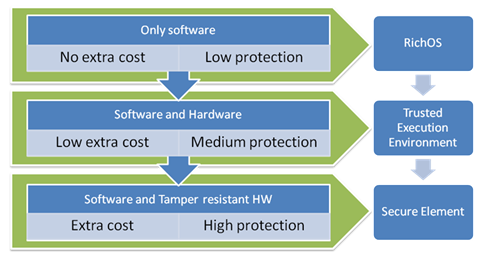
\includegraphics[scale=.6]{assets/tee-spot-img}
        \caption{Source: GlobalPlatform}
    \end{figure}
    \vfill
    \begin{block}{GlobalPlatform}
        Same as TCG, share some members.
    \end{block}
\end{frame}

\begin{frame}
    \frametitle{Why are they becoming important ?}

    \begin{block}{Always more}
        \begin{itemize}
            \item More mobile devices, everythong becomes connected.
            \item More users implies more malwares.
            \item More critical data to protect.
        \end{itemize}
        \medskip
        $\Rightarrow$ Hardware solutions
    \end{block}
    \vfill
    \begin{block}{When hardware alone is not enough}
        \begin{itemize}
            \item Create a link between software applications and hardware devices.\\
            \item Ensure that some software operations can be performed in a trusted environment.
        \end{itemize}
    \end{block}

    $\Rightarrow$ Former question: When are they used ?\\
    \medskip
    Source: GlobalPlatform
\end{frame}

\begin{frame}
    \frametitle{General scheme of a TEE}

    \begin{figure}[htb]
        \centering
        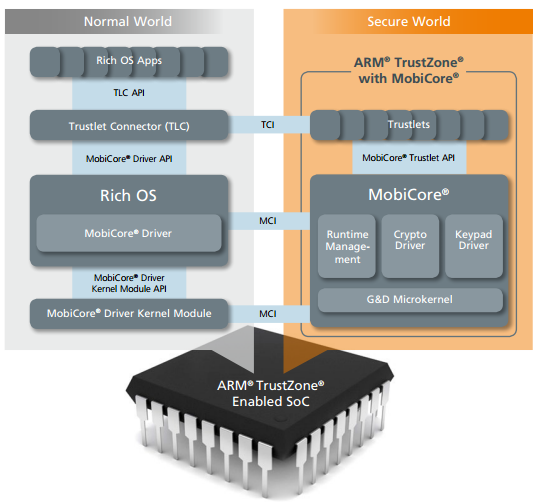
\includegraphics[scale=.5]{assets/tee}
        \caption{Source: Giesecke \& Devrient GmbH}
    \end{figure}
\end{frame}

\begin{frame}
    \frametitle{Security properties of TEE 1/2}

    \begin{itemize}
        \item {\bf Isolated Execution} -- Ensures applications execute completely isolated from and unhindered by others and guarantees that any code and data is protected at run-time.
        \vfill
        \item {\bf Secure Storage} -- Protects persistently stored data (e.g. cryptographic keys) belonging to a certain application from being accessed by other applications.
        \vfill
        \item {\bf Remote Attestation} -- Enables remote parties to ascertain they are dealing with a particular trusted application on a particular TEE.
    \end{itemize}
\end{frame}

\begin{frame}
    \frametitle{Security properties of TEE 2/2}

    \begin{itemize}
        \item {\bf Secure Provisioning} -- Enables communication by remote parties with a specific application on a specific TEE while protecting integrity and confidentiality.
        \vfill
        \item {\bf Trusted Path} -- A channel for the user to input data to the TEE and for the TEE to output data to the user; the channel protects against eavesdropping and tampering.
        \begin{itemize}
            \item Still the hardest one nowadays.
        \end{itemize}
    \end{itemize}

    \vfill
    Source: Vasudevan et al. [VOZ+12]
\end{frame}

\begin{frame}
    \frametitle{Formalization}

    \begin{block}{In natural language:}
        \begin{itemize}
            \item TEE Protection Profile from GlobalPlatform.
            \vfill
            \item Trustonic claims to be the first certified TEE.
            \begin{itemize}
                \item No info in the security target.
            \end{itemize}
        \end{itemize}
    \end{block}
    \vfill
    \begin{block}{Using mathematical formalism:}
        \begin{itemize}
            \item Some works on hypervisors proofs using coq [BBCL13], [VCJM+13]\\
            \begin{itemize}
                \item Not so far from TEE.
            \end{itemize}
            \vfill
            \item {\bf OASIS: on achieving a sanctuary for integrity and secrecy on untrusted platforms} [OGMN+13]\\
            \begin{itemize}
                \item Instruction set for TEE, seems to propose some formalization.
            \end{itemize}
        \end{itemize}
    \end{block}
\end{frame}

\begin{frame}
    \frametitle{Roots of Trust 1/2}

    Components are loaded sequentialy and each component checks the next component to launch against a known hash.

    $Hash_{n+1} = H(Hash_{n} + H(Component))$

    \begin{block}{Static Root of Trust Measurement}
        Begins with a trusted, static and immutable piece of code call the Core Root of Trust Measurement.\\
        It will check the BIOS before launch.

        \begin{figure}[htb]
            \centering
            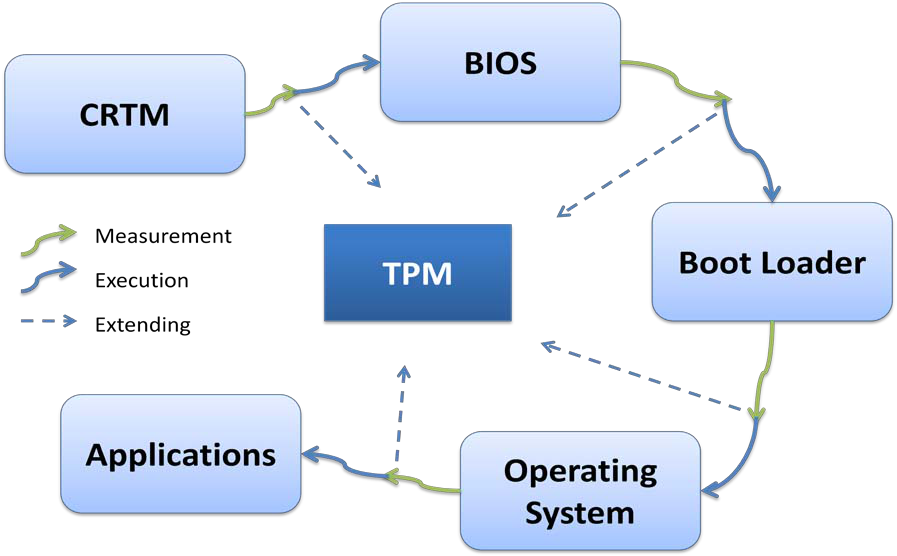
\includegraphics[scale=.15]{assets/srtm}
            \caption{Source: MSE Project Report}
        \end{figure}
    \end{block}
\end{frame}

\begin{frame}
    \frametitle{Roots of Trust 2/2}

    However, the boot chain is very large (3rd party modules such as network controllers must be checked to).
    \begin{itemize}
        \item Any little patch somewhere in the chain changes every hash after it since a hash depends on precedent hashes.\\
    \end{itemize}
    SRTM only gives load-time guarantee. If a library is modified between boot (aka. measurement) and its execution, attacks become feasible.

    \begin{block}{Dynamic Root of Trust Measurement}
        Rather than booting in a trusted state, a special instruction creates a safe execution environment.\\
        A short chain of trust is created from a trusted piece of code (like in SRTM).\\
        Part of the OS is also checked.\\
        Intended to allow loading of a hypervisor (such as Xen or VMWare ESX).\\
        Deeply dependant of the vendor implementation.
    \end{block}
\end{frame}

\section{Overview of existing TEE}

\begin{frame}
    \tableofcontents[currentsection]
\end{frame}

\begin{frame}
    \frametitle{TPM}

    \vfill
    \begin{itemize}
        \item First idea of a TEE by the TCG.
        \vfill
        \item Relies on a SRTM.
        \vfill
        \item Shelved in 2004 because TCB was becoming too large.
        \vfill
        \item New paradigm proposed in TPMv1.2 using DRTM.
        \begin{itemize}
            \item Used as a base by some vendors.
        \end{itemize}
    \end{itemize}
    \vfill
\end{frame}

\begin{frame}
    \frametitle{Flicker TEE [McCune et al. 2008]}

    \vfill
    \begin{itemize}
        \item Flicker takes advantage of DRTM but for much smaller amounts of code (Pieces of Application Logic -- PAL).
        \vfill
        \item Relies on the TPM idea.
        \vfill
        \item Flicker runs at highest level of privilege so PAL is protected from OS but not other way around.
    \end{itemize}
    \vfill
\end{frame}

\begin{frame}
    \frametitle{ARM TrustZone 1/2}

    \begin{figure}[htb]
        \centering
        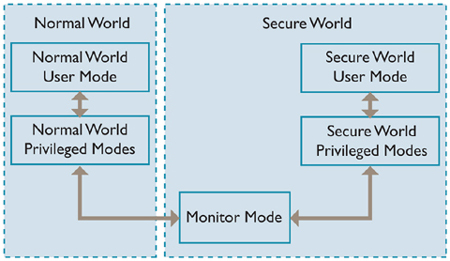
\includegraphics[scale=.4]{assets/TrustZone-Hardware-Architecture}
        \caption{Source: ARM website}
    \end{figure}
\end{frame}

\begin{frame}
    \frametitle{ARM TrustZone 2/2}

    \begin{figure}[htb]
        \centering
        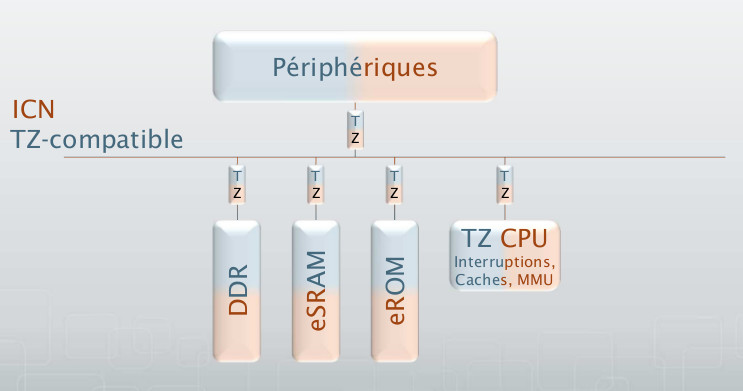
\includegraphics[scale=.4]{assets/TrustZone-Hardware-Architecture2}
        \caption{Source: SSTIC2013}
    \end{figure}
    \vfill
    \begin{itemize}
        \item CPU buses extended to a 33rd bit, signaling whether in secure mode.
        \vfill
        \item Signal exposed outside of the CPU to allow secure peripherals and secure RAM.
    \end{itemize}
    \vfill

\end{frame}

\begin{frame}
    \frametitle{Trustonic / Samsung KNOX}

    TrustZone is not very useful by itself due to only allowing one enclave (only one trustlet running at a time?).
    \vfill
    \begin{block}{Trustonic}
        Created in 2012 by 3 people of Giesecke \& Devrient, ARM and Trusted Logic Mobililty.\\
        Based on TrustZone (ARM) and MobiCore(G+D).
    \end{block}
    \vfill
    \begin{block}{Samsung KNOX [Samsung 2013]}
        Samsung Knox is similar, but also introduces secure boot.\\
        Relies (of course) on Android.
    \end{block}
    \vfill
\end{frame}

\begin{frame}
    \frametitle{Intel Identity Protection Technology [Carbin 2012]}

    \begin{itemize}
        \item Runs Java applet on separate CPU.
        \begin{itemize}
            \item Management Engine part of chipset so bound to physical hardware.
        \end{itemize}
        \vfill
        \item Applications currently available include:
        \begin{itemize}
            \item Key generation and storage (integrated with Windows Cryptographic API).
            \item One time password generation (VASCO MYDIGIPASS.COM).
            \item Secure PIN entry.
        \end{itemize}
        \item Video management for trusted display.
    \end{itemize}
\end{frame}

\begin{frame}
    \frametitle{Intel SGX}
    
    \begin{itemize}
        \item No publicly available hardware yet.
        \vfill
        \item Tightly integrated with CPU.
        \vfill
        \item As enclaves are built, the code is measured in a similar way to the TPM.
        \vfill
        \item Can be combined with IPT for trusted display.
    \end{itemize}
\end{frame}

\begin{frame}
    \frametitle{Performance}
    \begin{itemize}
        \item TPM:
        \begin{itemize}
            \item TPM is really slow, and only has slow communications bus to CPU.
            \item Flicker TEE code runs on main CPU so can be as fast and has access to as much RAM as OS will spare.
        \end{itemize}
        \vfill
        \item Trustzone (Trustonic, Samsung Knox):
        \begin{itemize}
            \item TEE code runs on main CPU so is as fast, but RAM may be limited.
        \end{itemize}
        \vfill
        \item Intel IPT:
        \begin{itemize}
            \item TEE code runs on separate CPU, which is moderately fast.
        \end{itemize}
        \vfill
        \item Intel SGX:
        \begin{itemize}
            \item TEE code runs on main CPU so is as fast, as much RAM as needed.
        \end{itemize}
    \end{itemize}
\end{frame}

\begin{frame}
    \frametitle{Flexibility}

    \begin{itemize}
        \item TPM functionality baked into hardware:
        \begin{itemize}
            \item Designed to be flexible but what is there cannot be changed.
        \end{itemize}
        \vfill
        \item Flicker allows arbitrary code to be run, but it does not have access to OS or drivers:
        \begin{itemize}
            \item As a result only computation and very simple I/O possible.
        \end{itemize}
        \vfill
        \item Intel IPT, Trustonic, Knox can run arbitrary code:
        \begin{itemize}
            \item But it has to be licensed by Intel, Trustonic, Samsung first.
        \end{itemize}
        \vfill
        \item SGX allows anyone to run arbitrary code.
    \end{itemize}
\end{frame}

\begin{frame}
    \frametitle{Conclusion: Comparison chart}

    \begin{figure}[htb]
        \centering
        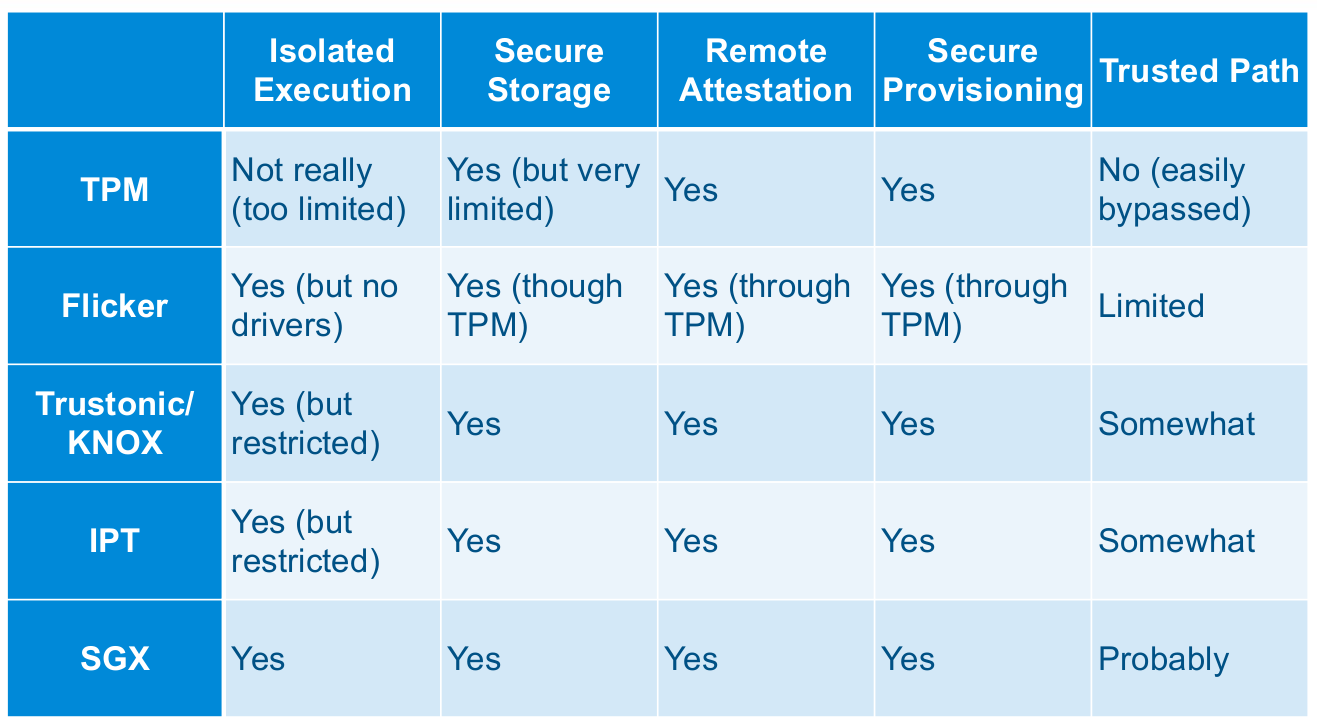
\includegraphics[scale=.33]{assets/chart}
        \caption{Source: Steven J. Murdoch - U. Cambridge}
    \end{figure}
\end{frame}

\end{document}
